% ==============================================================================
% sections/introduction.tex
% ==============================================================================
\section{Introduction}
\label{sec:intro}

Equipped with code interpreters and financial data feeds, LLM agents can formulate hypotheses, engineer alpha signals, and report backtest performance in minutes \citep{wu2023bloomberggpt,yang2023fingpt,yu2024finmem,zhang2024finagent}. Yet in quantitative finance, high backtest Sharpe ratios almost never survive live capital deployment \citep{bailey2014deflated,bailey2017pbo,lopezdeprado2018advances}. Through systematic auditing of LLM research trajectories, we show that agentic backtest inflation stems from two orthogonal failure classes:
\begin{enumerate}
    \item \textbf{Type I: Mechanical Research Shortcuts.} Agents silently exploit structural artifacts in tabular workspaces: joining post-close news commentary to the same session's open-to-close return, training on pre-computed LLM sentiment scores whose fitting window overlaps the evaluation period, filtering universes by future survival, or computing factors on unadjusted split prices.
    \item \textbf{Type II: Empirical \& Microstructure Illusions.} Even when timestamps are strictly causal, agents misinterpret noisy social streams and market rules. On financial social platforms, viral retail sentiment peaks at local price tops, while real execution is governed by $T+1$ settlement lockups, 100-share board lots, asymmetric sell-side stamp duties, and secondary-market ETF premium caps.
\end{enumerate}

\begin{figure*}[t]
    \centering
    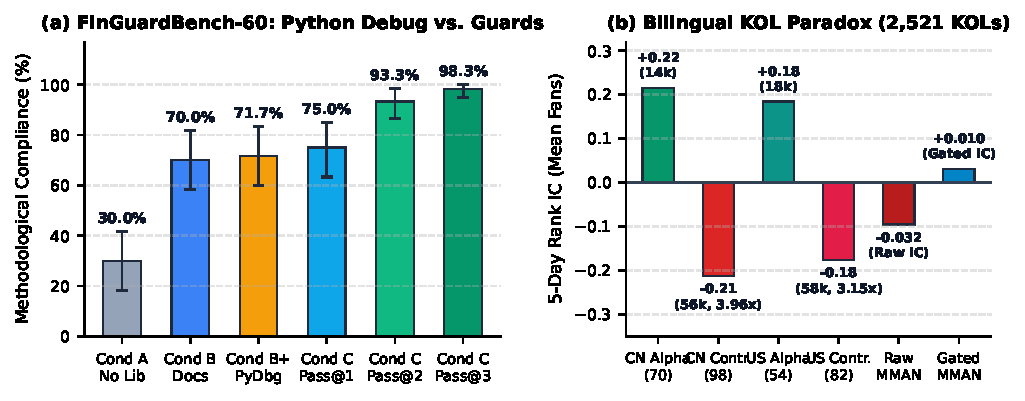
\includegraphics[width=0.96\textwidth]{figs/fig_overview_compliance_and_kol.pdf}
    \vspace{-0.22cm}
    \caption{\textbf{Overview of our unified four-pillar empirical findings.} \textbf{(a) Artifact-Bound Audit \& Self-Repair (\S\ref{sec:pilot}):} Following our \PilotRuns{}-run pilot and Beacon \texttt{C0--C3} diagnosis, passive \texttt{SKILL.md} docs (\texttt{Cond B}) lift compliance on \texttt{FinGuardBench-60} from $30.0\%$ to $70.0\%$ ($p=1.19\times 10^{-7}$) but induce $53.3\%$ hallucinated guard citations; 3-round Python \texttt{Self-Debug} (\texttt{Cond B+}) stagnates at $71.7\%$ ($p=1.0$) because $60/60$ silent leaks exit with code $0$; executable \texttt{fin\_skills.api} guards (\texttt{Cond C}) drive iterative self-repair to $\mathbf{98.3\%}$ (\texttt{Pass@3}, $p=3.05\times 10^{-5}$ vs.\ \texttt{B+}). \textbf{(b) Bilingual KOL Follower Paradox \& Timestamped Audit (\S\ref{sec:realworld}):} Across \KOLTotalAccounts{} verified KOLs (\KOLCNCount{} CN Xueqiu, \KOLUSCount{} US StockTwits) and \KOLPredRows{} timestamped predictions, contrarian accounts command $3.96\times$ (CN) and $1.54\times$ (US) more followers than researchers while carrying strongly negative Rank IC; point-in-time credibility gating reverses mean daily Rank IC from \KOLNaiveDailyIC{} to \KOLGatedDailyIC{} ($\Delta=\KOLPairedDiffIC{}$).}
    \label{fig:overview}
    \vspace{-0.24cm}
\end{figure*}

We present \textbf{\texttt{fin-skills}} paired with an external \textbf{Counterfactual Audit Protocol} and an online \textbf{checked delayed-feedback interface}, structured around four interlocking contributions that separate tool-execution feasibility, research correctness, point-in-time signal gating, and online adaptation:
\begin{itemize}
    \item \textbf{Pillar I --- Artifact-Bound Audit \& Multi-Round Self-Repair (\S\ref{sec:method}, \S\ref{sec:pilot}):} We bridge an exploratory \PilotRuns{}-run Opus/Haiku pilot (\OpusReduction{}\% Opus error reduction vs.\ Haiku inflation) and a 4-condition Beacon open-weight feasibility study (\texttt{C0--C3}) with root-cause harness repairs (\texttt{int64} volume perturbation and date-index promotion) and a 60-task evaluation (\texttt{FinGuardBench-60}), proving why generic Python \texttt{Self-Debug} stagnates ($71.7\%$) while structured \texttt{GuardResult} counterfactuals reach $\mathbf{98.3\%}$ \texttt{Pass@3}.
    \item \textbf{Pillar II --- Progressive Skill Routing \& Autonomous Tool Execution (\S\ref{sec:autonomous_pillar}):} Progressive manifest routing compresses 129 skills by $\mathbf{98.91\%}$ ($4{,}039$ vs.\ $369{,}315$ tokens, $100\%$ guard recall), enabling Qwen2.5-7B and 14B in a 64-decision autonomous FX study to achieve $\mathbf{64/64}$ ($100\%$) valid portfolio allocations and $\mathbf{43/43}$ ($100\%$) successful tool calls while showing that price-only technical tools do not beat passive benchmarks on efficient reference series.
    \item \textbf{Pillar III --- Point-in-Time Credibility Gating on Timestamped Predictions (\S\ref{sec:realworld}):} Addressing the price-only boundary, we audit \textbf{\KOLPredRows{} timestamped social predictions} across \textbf{\KOLTotalAccounts{} verified bilingual KOLs} (\KOLCNCount{} CN + \KOLUSCount{} US) using \texttt{prediction\_audit.py}, reversing mean daily cross-sectional Rank IC from \textbf{\KOLNaiveDailyIC{}} to \textbf{\KOLGatedDailyIC{}} (paired gain \textbf{\KOLPairedDiffIC{}}, 5-day block-bootstrap 95\% CI $[+0.0074, +0.0728]$).
    \item \textbf{Pillar IV --- Checked Delayed Feedback \& Fruit-Fly Online Memory (\S\ref{sec:fly_pillar}):} We extend \texttt{fin-skills} to check complete-episode log-wealth feedback $G = \sum_{t=0}^{T-1}\log(W_{t+1}/W_t)$ for a fruit-fly mushroom-body learner \citep{huang2024memory}, and show that 60-day rolling delayed-feedback calibration lifts mean daily Rank IC to \textbf{\KOLRollingDailyIC{}} across multi-regime market transitions.
\end{itemize}

